\subsection{Trapezium}

\subsubsection{Area}
\begin{figure}
    \centering

    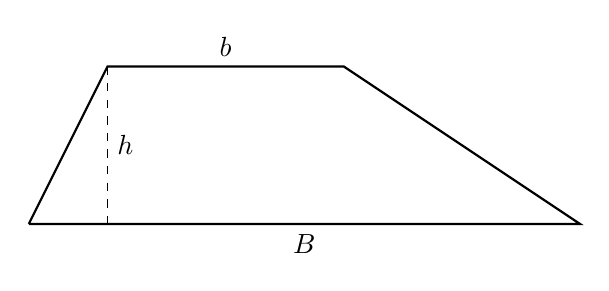
\begin{tikzpicture}
        \coordinate (A) at (0, 0);
        \coordinate (B) at (7, 0);
        \coordinate (C) at (4, 2);
        \coordinate (D) at (1, 2);
        \coordinate (O) at (1, 0);

        \draw[thick] (A) -- node[anchor=north] { $B$ } (B) -- (C) -- node[anchor=south] { $b$ } (D) -- (A);
        \draw[dashed] (D) -- node[anchor=west] { $h$ } (O);

    \end{tikzpicture}
\end{figure}
\[
    A = \frac{(B + b)h}{2}
\]

